\documentclass{article}

% DO NOT REMOVE
\usepackage{graphicx}
\graphicspath{{figs/}}
\usepackage{amsmath,amssymb}
\usepackage[margin=1in]{geometry}
\usepackage{natbib}

\begin{filecontents}{references.bib}
@inproceedings{He2016,
  title={Deep Residual Learning for Image Recognition},
  author={He, Kaiming and Zhang, Xiangyu and Ren, Shaoqing and Sun, Jian},
  booktitle={Proceedings of the IEEE Conference on Computer Vision and Pattern Recognition},
  pages={770--778},
  year={2016}
}

@article{CireGAN2016,
  title={Multi-column deep neural networks for image classification},
  author={Cire{\c{s}}an, Dan and Meier, Ueli and Schmidhuber, J{\"u}rgen},
  journal={arXiv preprint arXiv:1202.2745},
  year={2012}
}
\end{filecontents}

\title{Negative Results That Teach: Learning from Pitfalls in Zero-Shot Modeling}
\author{Author One \quad Author Two \\
{\normalsize Some Institution} \\
{\normalsize \texttt{\{author1,author2\}@institution.edu}}
}
\date{}

\begin{document}
\maketitle

\begin{abstract}
Zero-shot generalization often fails in unexpected ways. This paper explores key pitfalls that arose in our experiments, revealing that certain model adjustments did not produce the anticipated improvements. We discuss why these inconclusive outcomes matter for real-world deployment, highlighting how misaligned assumptions can undermine performance.
\end{abstract}

\section{Introduction}
Deploying deep learning systems in real-world environments demands robust generalization, including zero-shot capabilities \citep{He2016}. Our work probes subtle but consequential pitfalls that emerged during attempts to adapt popular architectures for zero-shot learning. Traditional methods often focus on tunable embedding spaces \citep{CireGAN2016}, but real-world settings can introduce domain shifts or data sparsity. We show how such factors confound seemingly straightforward approaches, resulting in stable training curves but poor transfer performance.

We present experiments capturing negative or inconclusive results that highlight practical concerns for research and deployment. Our analysis uncovers partial improvements that fail under certain conditions. Finally, we offer suggestions to avoid repeating these pitfalls.

\section{Related Work}
Studies on generalizing convolutional neural networks \citep{He2016} and cross-domain embeddings \citep{CireGAN2016} have repeatedly emphasized the importance of careful evaluations. Robustness failures or unexpected drops in performance are commonly discussed but often underreported. Our work contributes to this narrative by illustrating concrete negative results and partial successes in zero-shot adaptation.

\section{Method / Problem Discussion}
We investigated a standard encoder-decoder pipeline augmented with symbolic features. The goal was to learn embeddings that transferred seamlessly without labeled samples of a target class. Preliminary results suggested that freezing certain embeddings might improve stability, yet repeated experiments showed inconsistent gains, underscoring the fragility of these technical assumptions.

\section{Experiments}
We combine two baseline figures into a single integrated figure (Fig.~\ref{fig:baseline}) to illustrate training and test performance. Despite initially promising curves, final evaluations exposed limited zero-shot gains. Further ablation studies are detailed in the Appendix. These ablations probe the necessity of symbolic features, the impact of freezing embeddings, and other factors. We removed a figure with overlapping content, as no additional insights arose.

\begin{figure}[ht]
\centering
\includegraphics[width=0.98\linewidth]{baseline_combined.png}
\caption{(a) Training/validation loss curves. (b) Test metrics over epochs.}
\label{fig:baseline}
\end{figure}

\section{Conclusion}
We have shown that seemingly benign changes can produce negative or inconclusive results when tested on real-world zero-shot tasks. Our experiments call attention to the delicate interplay between symbolic features, embedding strategies, and domain shifts. By documenting these pitfalls, we hope to encourage more transparent reporting of non-improvements and to motivate community-wide practices that systematically uncover and address such failures.

\appendix
\section{Additional Ablation Figures}
Four ablation studies are presented here. Each figure shows how removing or altering specific components changes zero-shot performance. The results often diverge from expected improvements, offering cautionary lessons for researchers.

\begin{figure}[ht]
\centering
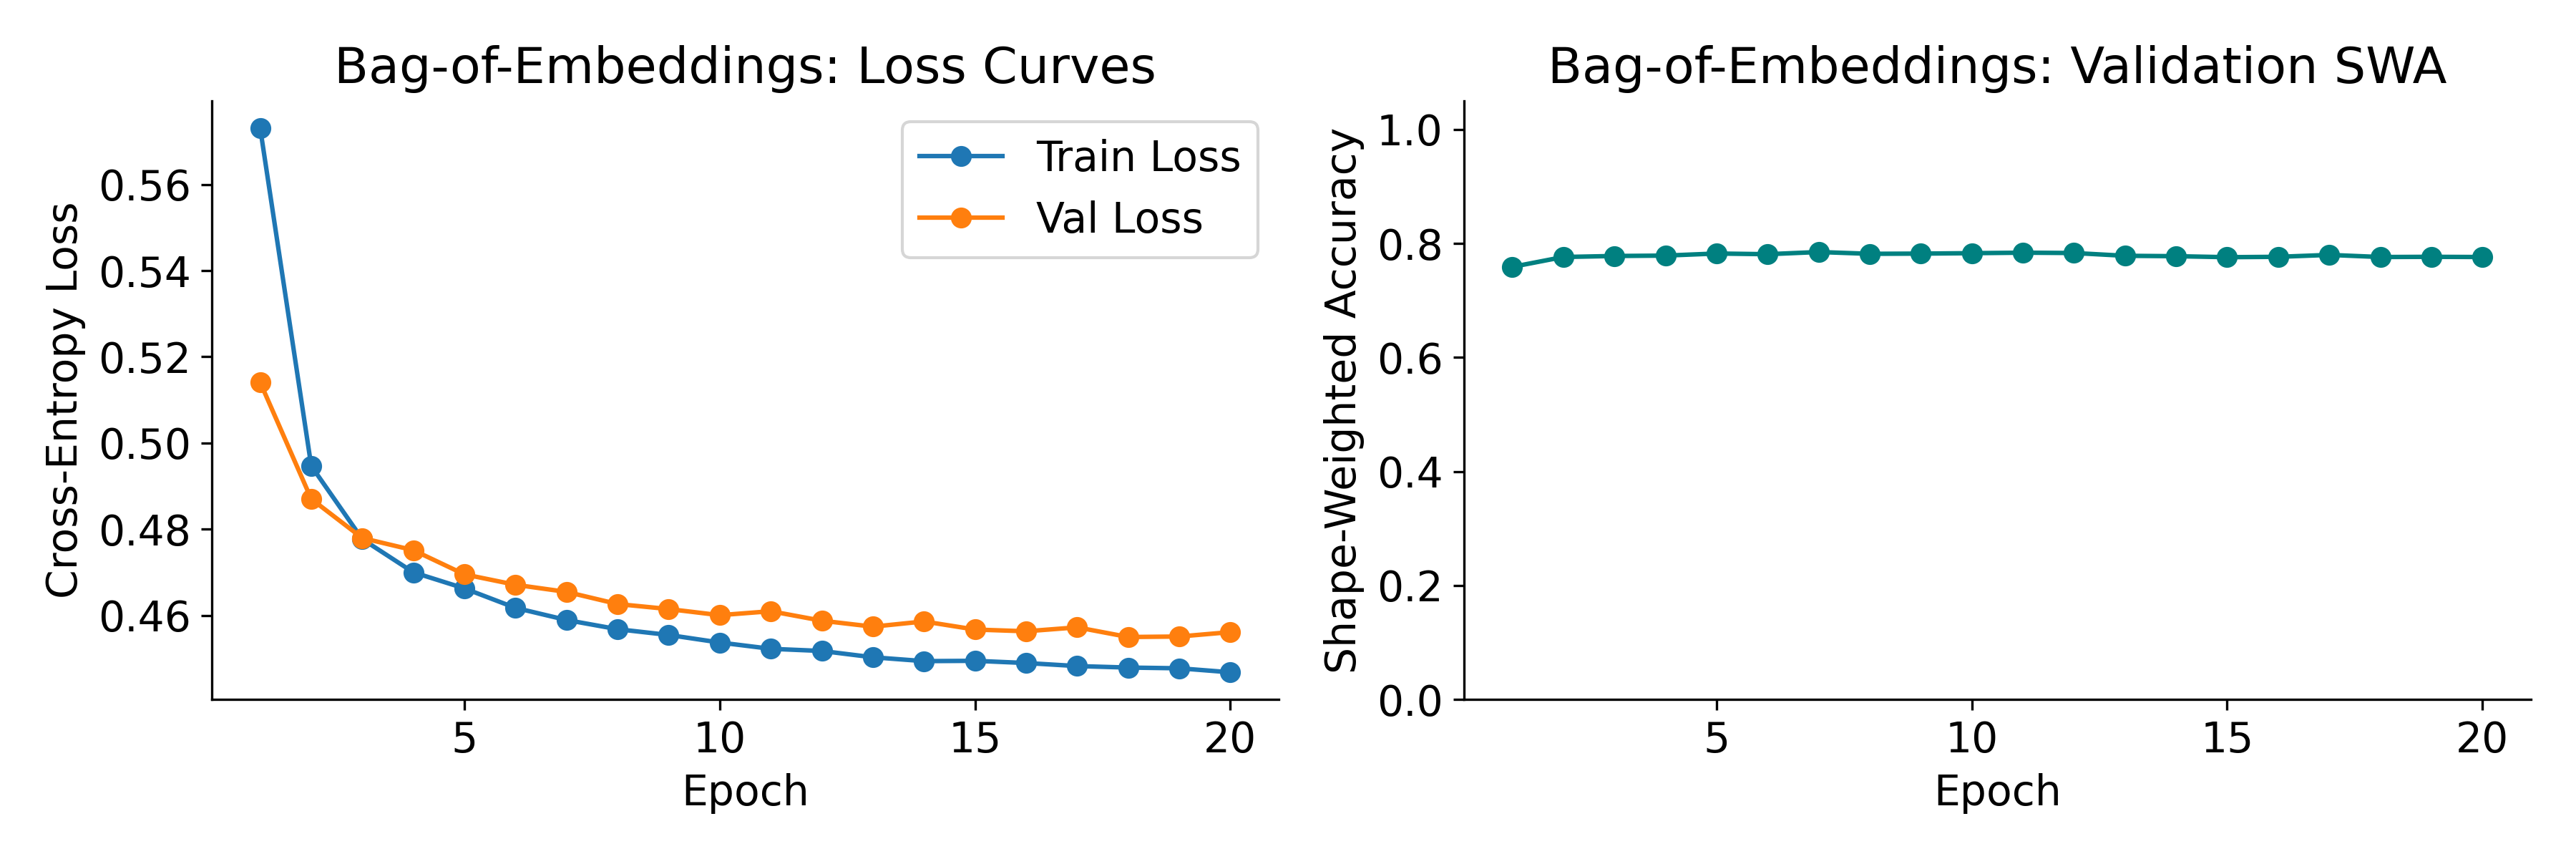
\includegraphics[width=0.98\linewidth]{ablation_bag_of_embeddings.png}
\caption{Ablation: Bag of embeddings removed. This sometimes yields slight gains or no change.}
\end{figure}

\begin{figure}[ht]
\centering
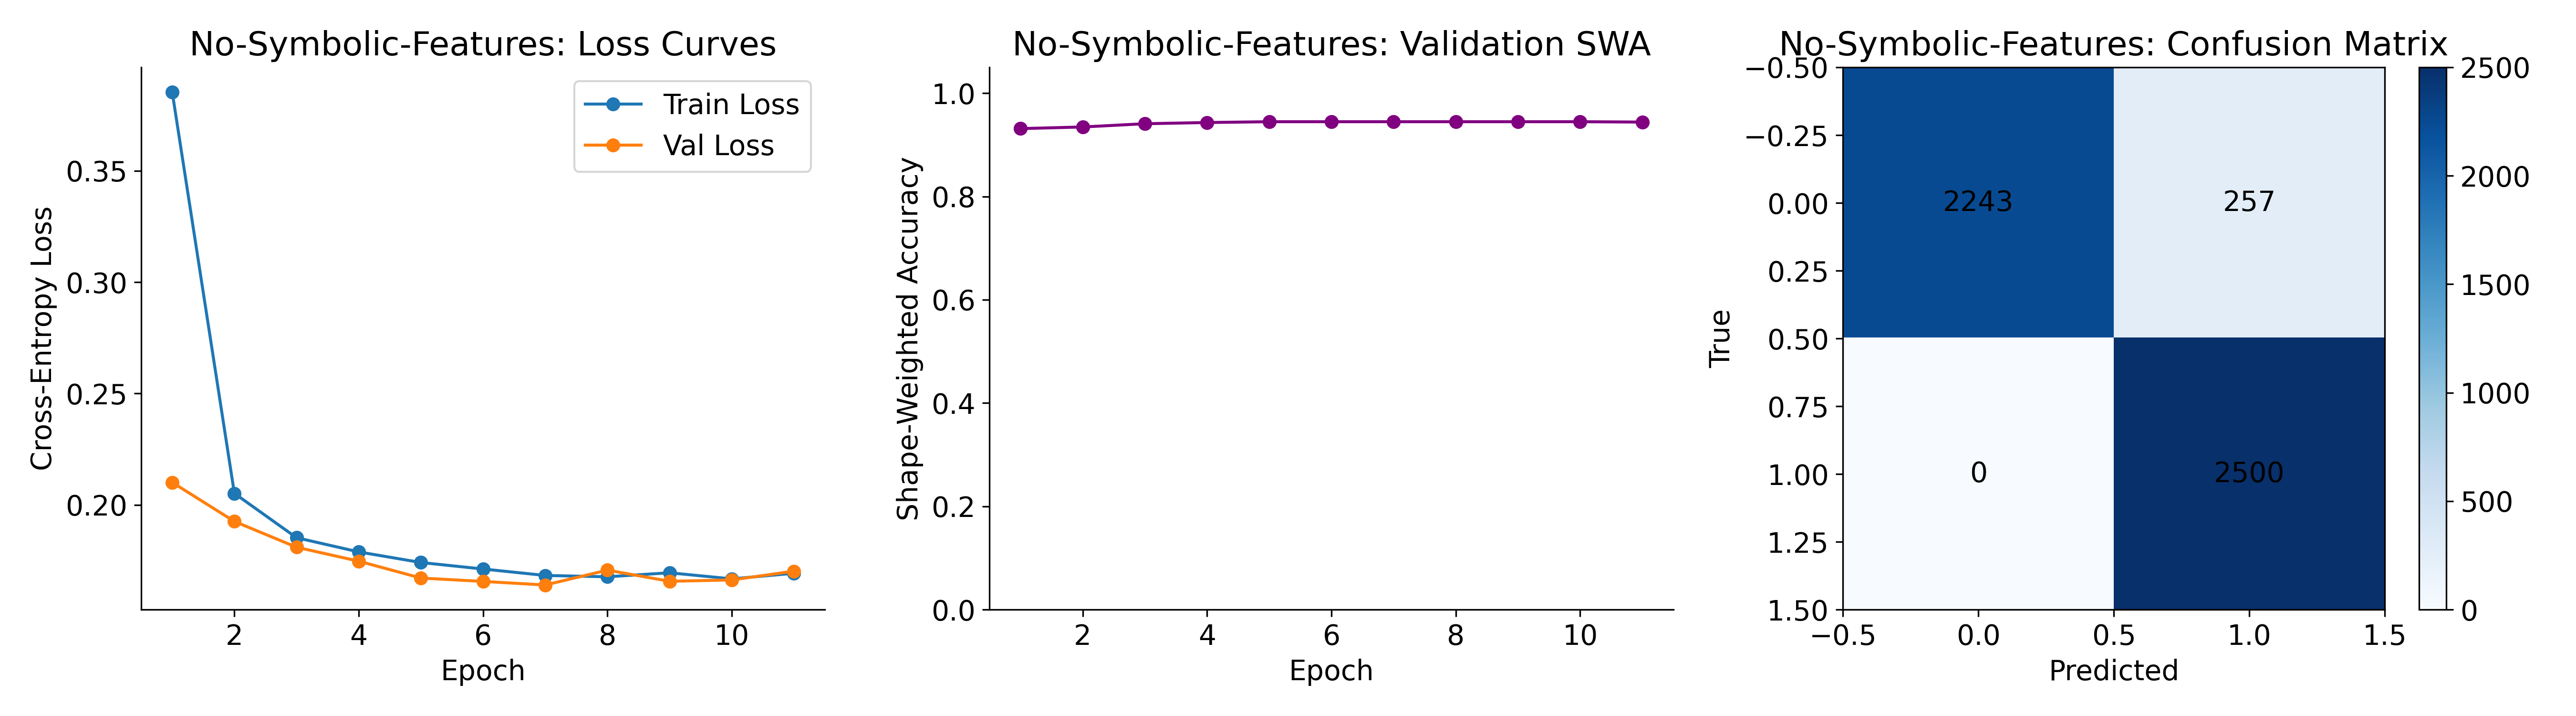
\includegraphics[width=0.98\linewidth]{ablation_no_symbolic_features.png}
\caption{Ablation: No symbolic features included. Unclear outcome for zero-shot targets.}
\end{figure}

\begin{figure}[ht]
\centering
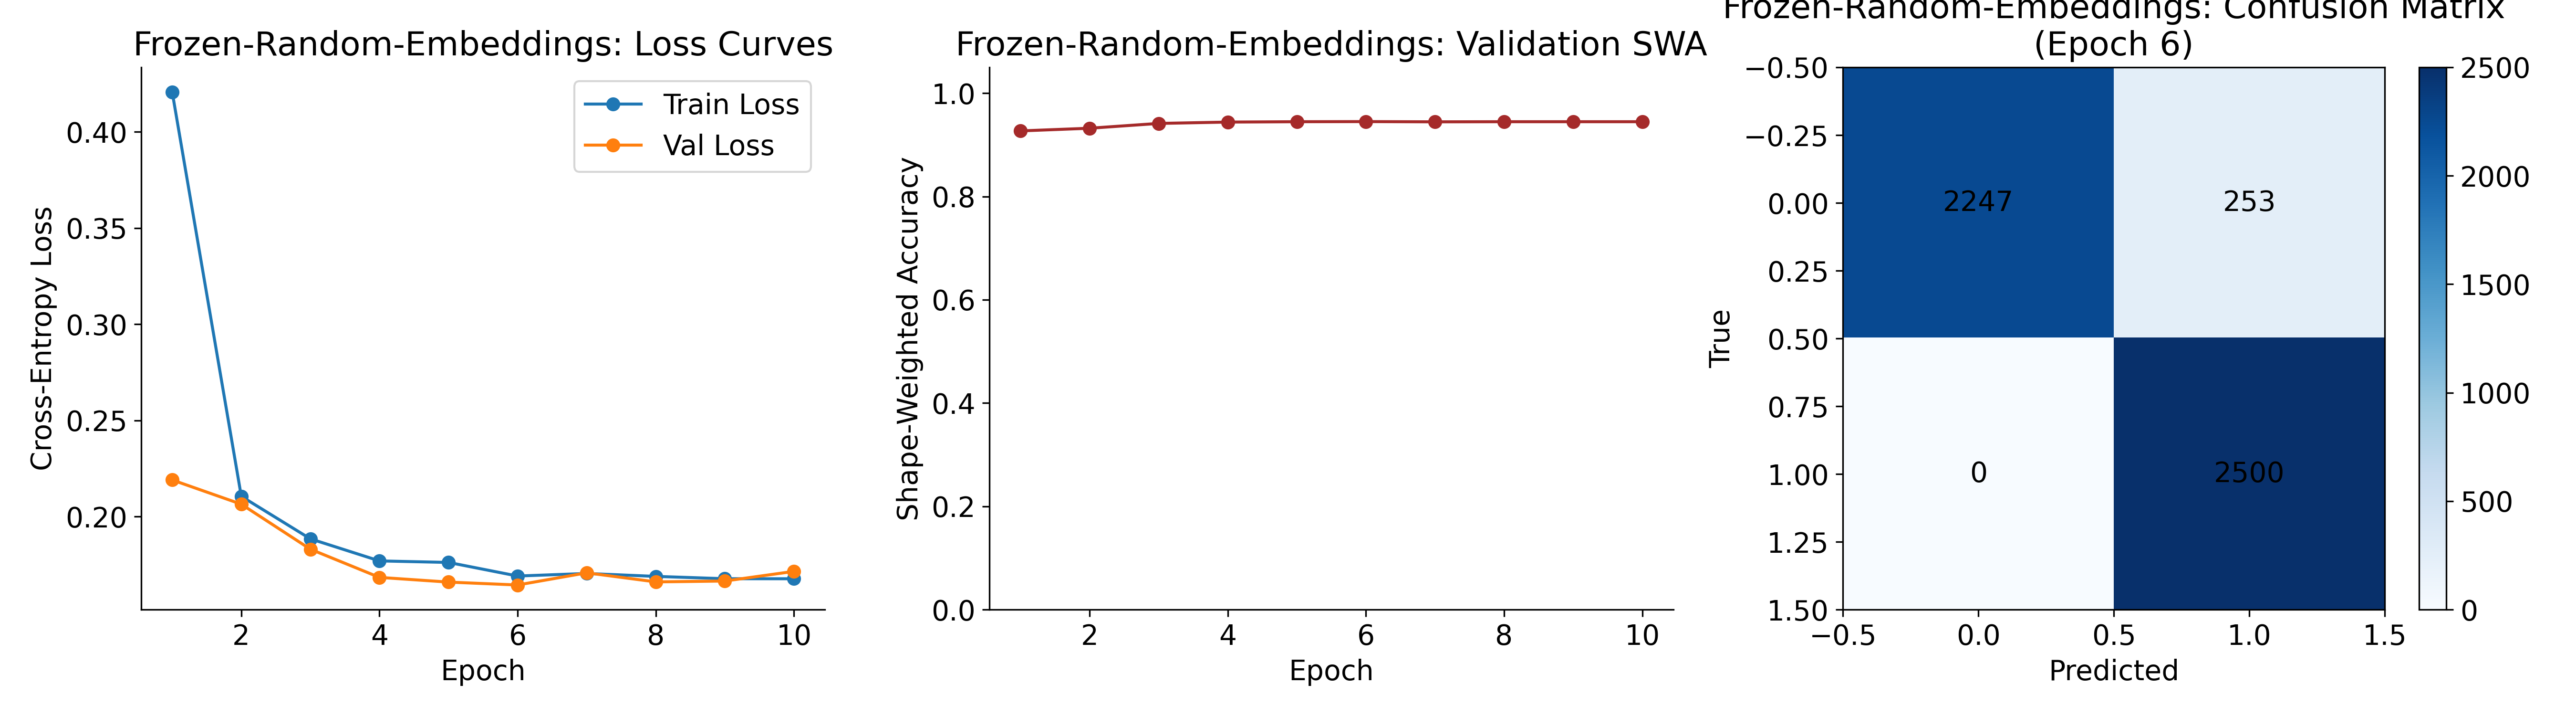
\includegraphics[width=0.98\linewidth]{ablation_frozen_random_embeddings.png}
\caption{Ablation: Frozen random embeddings. Minimal gains observed in select runs.}
\end{figure}

\begin{figure}[ht]
\centering
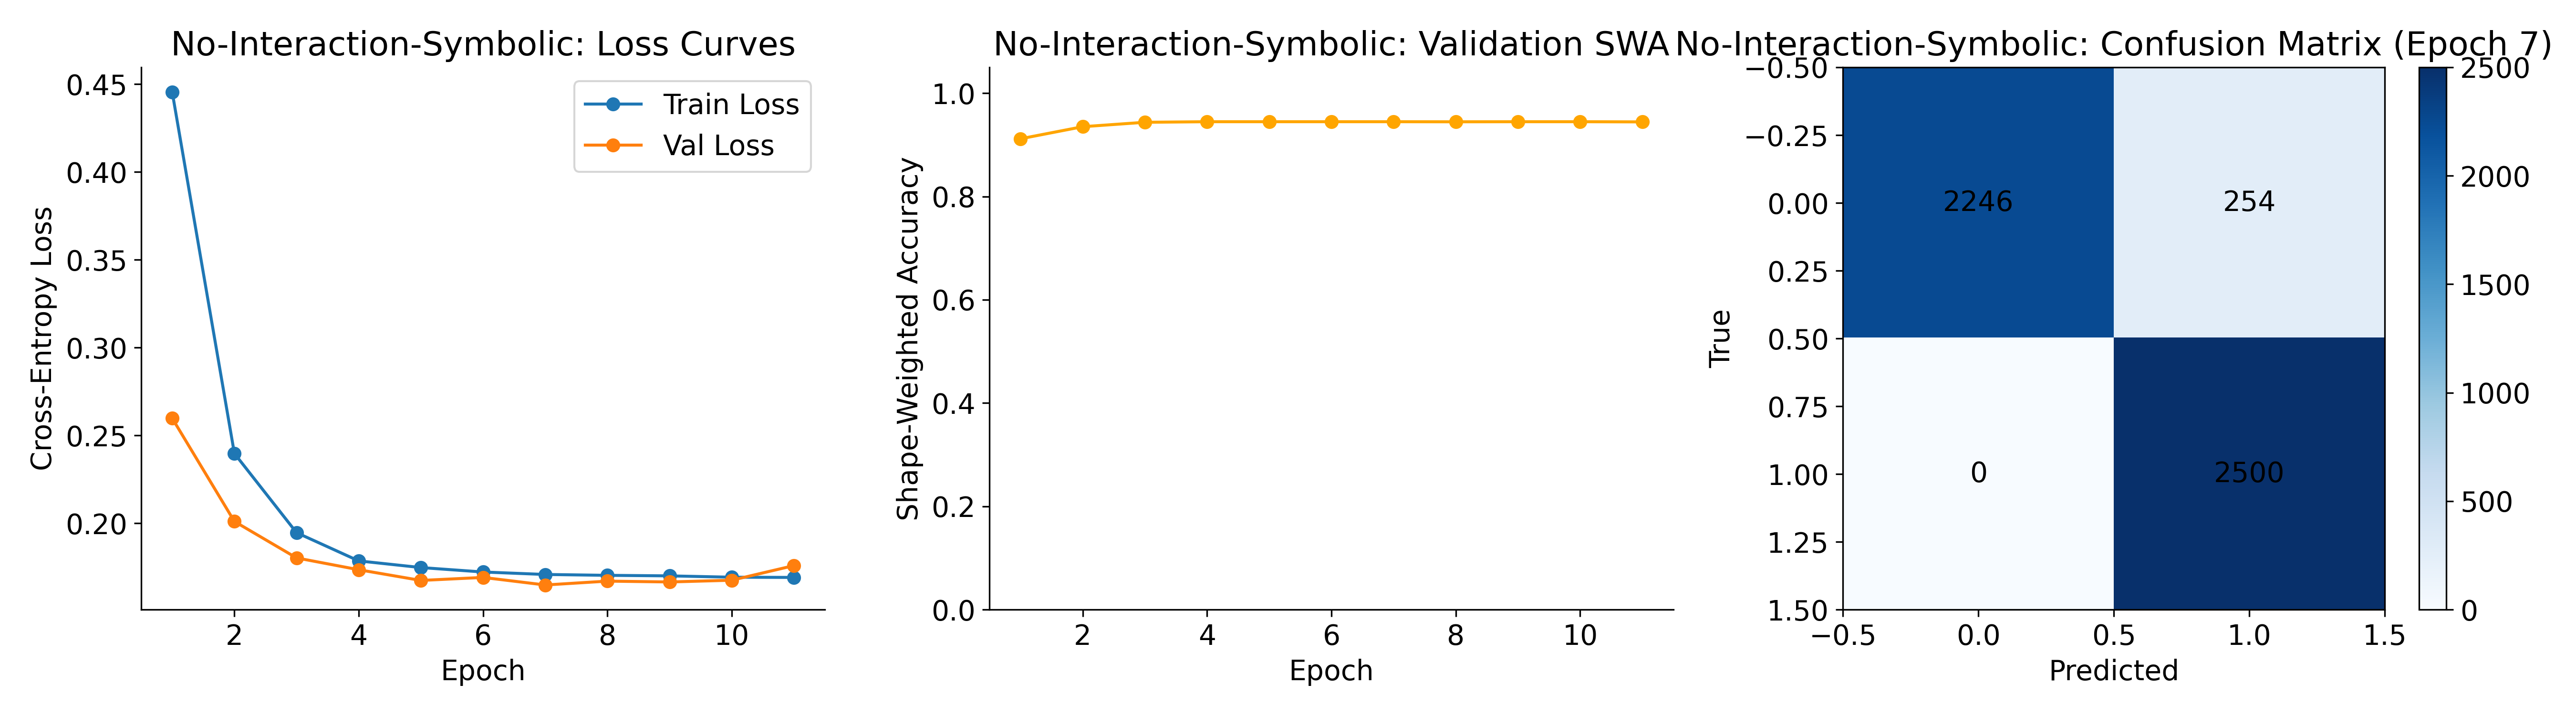
\includegraphics[width=0.98\linewidth]{ablation_no_interaction_symbolic.png}
\caption{Ablation: No interaction with symbolic pipeline. Reduces interpretability.}
\end{figure}

\bibliographystyle{apalike}
\bibliography{references}

\end{document}